% Options for packages loaded elsewhere
\PassOptionsToPackage{unicode}{hyperref}
\PassOptionsToPackage{hyphens}{url}
%
\documentclass[
  12pt,
]{article}
\usepackage{amsmath,amssymb}
\usepackage{lmodern}
\usepackage{iftex}
\ifPDFTeX
  \usepackage[T1]{fontenc}
  \usepackage[utf8]{inputenc}
  \usepackage{textcomp} % provide euro and other symbols
\else % if luatex or xetex
  \usepackage{unicode-math}
  \defaultfontfeatures{Scale=MatchLowercase}
  \defaultfontfeatures[\rmfamily]{Ligatures=TeX,Scale=1}
\fi
% Use upquote if available, for straight quotes in verbatim environments
\IfFileExists{upquote.sty}{\usepackage{upquote}}{}
\IfFileExists{microtype.sty}{% use microtype if available
  \usepackage[]{microtype}
  \UseMicrotypeSet[protrusion]{basicmath} % disable protrusion for tt fonts
}{}
\makeatletter
\@ifundefined{KOMAClassName}{% if non-KOMA class
  \IfFileExists{parskip.sty}{%
    \usepackage{parskip}
  }{% else
    \setlength{\parindent}{0pt}
    \setlength{\parskip}{6pt plus 2pt minus 1pt}}
}{% if KOMA class
  \KOMAoptions{parskip=half}}
\makeatother
\usepackage{xcolor}
\usepackage[margin=1in]{geometry}
\usepackage{longtable,booktabs,array}
\usepackage{calc} % for calculating minipage widths
% Correct order of tables after \paragraph or \subparagraph
\usepackage{etoolbox}
\makeatletter
\patchcmd\longtable{\par}{\if@noskipsec\mbox{}\fi\par}{}{}
\makeatother
% Allow footnotes in longtable head/foot
\IfFileExists{footnotehyper.sty}{\usepackage{footnotehyper}}{\usepackage{footnote}}
\makesavenoteenv{longtable}
\usepackage{graphicx}
\makeatletter
\def\maxwidth{\ifdim\Gin@nat@width>\linewidth\linewidth\else\Gin@nat@width\fi}
\def\maxheight{\ifdim\Gin@nat@height>\textheight\textheight\else\Gin@nat@height\fi}
\makeatother
% Scale images if necessary, so that they will not overflow the page
% margins by default, and it is still possible to overwrite the defaults
% using explicit options in \includegraphics[width, height, ...]{}
\setkeys{Gin}{width=\maxwidth,height=\maxheight,keepaspectratio}
% Set default figure placement to htbp
\makeatletter
\def\fps@figure{htbp}
\makeatother
\setlength{\emergencystretch}{3em} % prevent overfull lines
\providecommand{\tightlist}{%
  \setlength{\itemsep}{0pt}\setlength{\parskip}{0pt}}
\setcounter{secnumdepth}{-\maxdimen} % remove section numbering
\usepackage{natbib}
\bibliographystyle{abbrvnat}
\setcitestyle{authoryear, open={((},close={)}}
\usepackage{indentfirst}
\ifLuaTeX
  \usepackage{selnolig}  % disable illegal ligatures
\fi
\IfFileExists{bookmark.sty}{\usepackage{bookmark}}{\usepackage{hyperref}}
\IfFileExists{xurl.sty}{\usepackage{xurl}}{} % add URL line breaks if available
\urlstyle{same} % disable monospaced font for URLs
\hypersetup{
  pdftitle={Relationship between lifestyle risk factors and development of prediabetes or diabetes, based on BRFSS 2015 questionnaire},
  pdfauthor={Tianyang Jiang, Changhao Jiang, Liuye Huang},
  hidelinks,
  pdfcreator={LaTeX via pandoc}}

\title{Relationship between lifestyle risk factors and development of
prediabetes or diabetes, based on BRFSS 2015 questionnaire}
\author{Tianyang Jiang, Changhao Jiang, Liuye Huang}
\date{June 01, 2023}

\begin{document}
\maketitle
\begin{abstract}
This paper is about diabetes\ldots{}
\end{abstract}

\textbf{Keywords:} Diabetes, Lifestyle intervention, Causal inference,
R-learner, PC algorithm, Regression adjustment

\hypertarget{background}{%
\subsection{Background}\label{background}}

\hypertarget{data-description}{%
\subsection{Data Description}\label{data-description}}

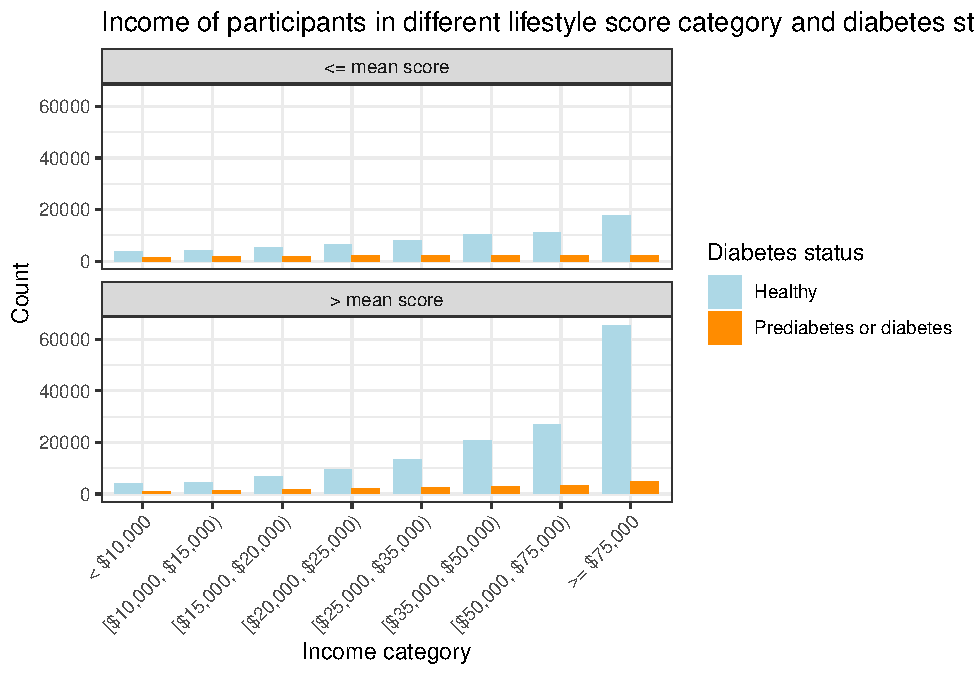
\includegraphics{template_files/figure-latex/unnamed-chunk-3-1.pdf}
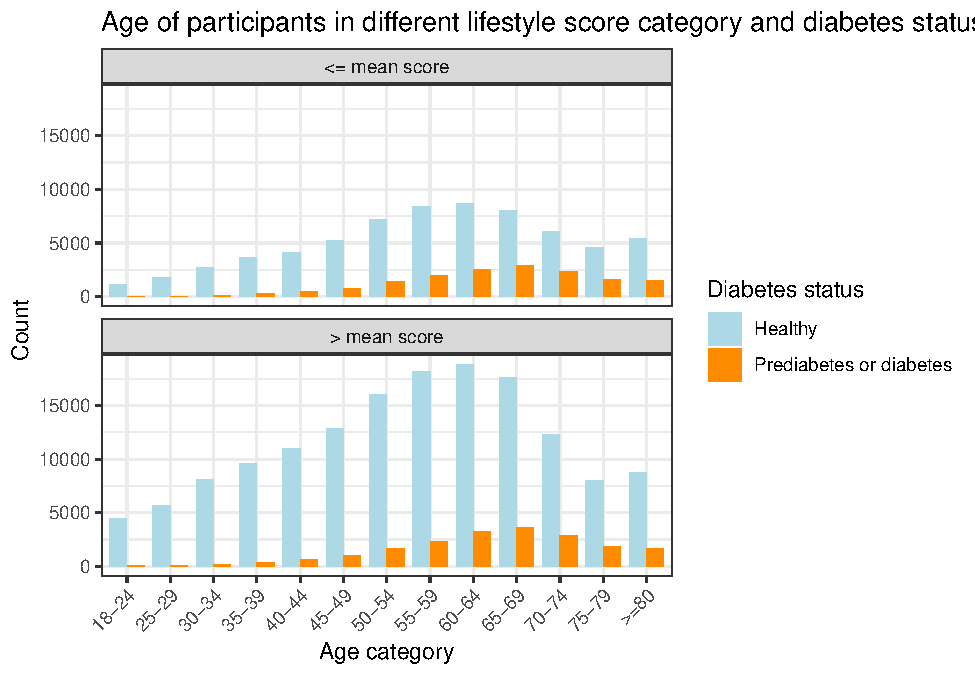
\includegraphics{template_files/figure-latex/unnamed-chunk-3-2.pdf}
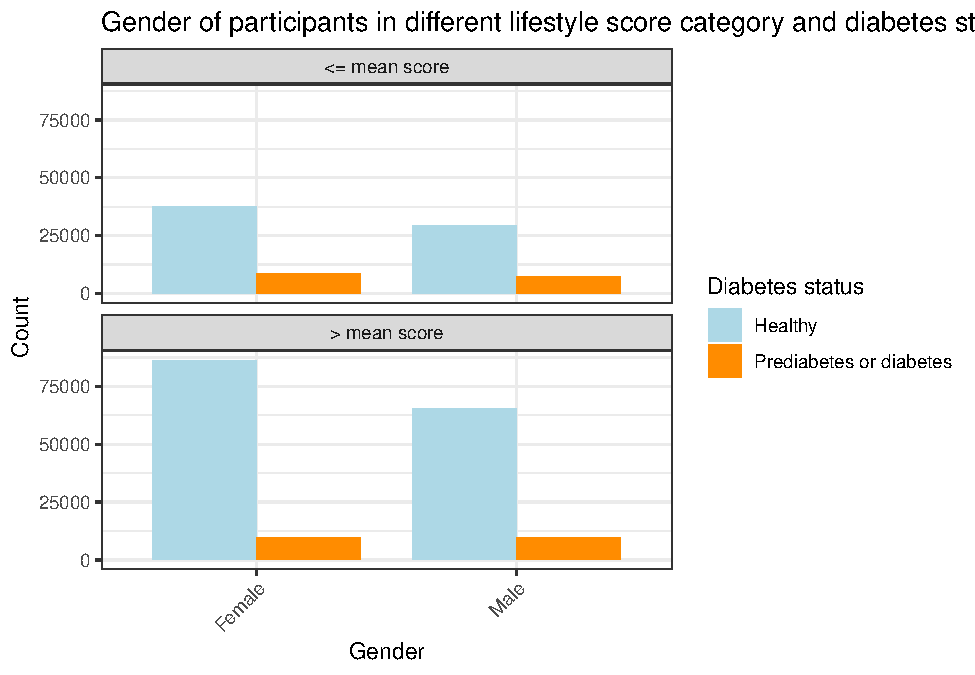
\includegraphics{template_files/figure-latex/unnamed-chunk-3-3.pdf}

\hypertarget{statistical-methods}{%
\subsection{Statistical Methods}\label{statistical-methods}}

{[}Explain the statistical methods employed in the analysis, such as
linear regression, Bayesian analysis, etc. Provide a brief rationale for
their selection.{]}

\hypertarget{find-scores-with-random-forest}{%
\subsubsection{Find Scores with Random
Forest}\label{find-scores-with-random-forest}}

\hypertarget{build-dag-with-pc-algorithm-and-literature-review}{%
\subsubsection{Build DAG with PC Algorithm and Literature
Review}\label{build-dag-with-pc-algorithm-and-literature-review}}

\hypertarget{logistic-regression-with-adjustment}{%
\subsubsection{Logistic Regression with
Adjustment}\label{logistic-regression-with-adjustment}}

We consider the variable diabetes as the outcome variable, denoted as
\(Y\), and the variable score as the treatment variable, denoted as
\(X\). Our objective is to estimate the average causal effect of the
score on diabetes, which can be expressed as \(E[Y(X=1)] - E[Y(X=0)]\).

Before estimating the causal effect, it is essential to examine the
association between diabetes and scores. In this case, diabetes takes
the value 1 if a person has diabetes and 0 if a person does not have
diabetes. Additionally, we assume a linear relationship between the
log-odds of diabetes and scores. Hence, it is reasonable to employ a
simple logistic model to capture their relationship.

We consider the following model:
\(\text{log}(\frac{p}{1-p}) = \beta_0 + \beta_1 X\), where \(p\)
represents the probability of an individual having diabetes,
\(\frac{p}{1-p}\) represents the odds, and \(\text{log}(\frac{p}{1-p})\)
represents the log-odds. In this model, \(X\) corresponds to the score,
and \(\beta\) represents the corresponding coefficients.

Based on the Directed Acyclic Graph (DAG) shown in Graph 1, we observe
three confounding paths. These paths indicate that confounding
variables, namely age, gender, and income, simultaneously connect
diabetes and scores. Consequently, estimating the effect of the score
without accounting for these confounding variables would introduce bias.
Therefore, it is necessary to determine whether controlling for these
confounders would yield better estimates of the parameter of interest.

Using the adjustment criterion proposed by Shpitser et al.~(2012), we
conclude that adjusting for the three variables (denoted as
\(Z=\{Z_1, Z_2, Z_3\}\), where \(Z_1\) represents age, \(Z_2\)
represents income, and \(Z_3\) represents gender) is sufficient. This
adjustment blocks all spurious paths from scores to diabetes and
addresses confounding for the three variables. Moreover, it also blocks
the confounding path for the variable education. Importantly, this
adjustment does not block any of the causal paths from scores to
diabetes and does not open any spurious paths. Consequently, we can
utilize the non-parametric identification result from the observational
distribution, which states that \(E[Y(X=x)] = E[E[Y|X=x,Z]]\). Notably,
when \(Z\) satisfies the adjustment criterion, the conditional
ignorability assumption holds, i.e., \(Y_x \perp\!\!\!\perp X |Z\). This
assumption aids in recovering the causal effect and improving the
accuracy of the estimation, as highlighted by Cinelli et al.~(2022).

Since we assume a linear relationship between the log-odds of diabetes
and scores, age, income, and gender, which aligns with the
aforementioned model, the logistic regression for confounding adjustment
can be written as
\(\text{log}(\frac{p}{1-p}) = \beta_0 + \beta_1 X + \gamma_1 Z_1 + \gamma_2 Z_2 + \gamma_3 Z_3\),
where \(\gamma\) represents the corresponding coefficients.
Consequently, the average causal effect corresponds to the regression
coefficient \(\beta_1\) (Cinelli et al., 2022).

\begin{longtable}[]{@{}lccc@{}}
\caption{Adjustment Results}\tabularnewline
\toprule()
& Estimate & 2.5 \% & 97.5 \% \\
\midrule()
\endfirsthead
\toprule()
& Estimate & 2.5 \% & 97.5 \% \\
\midrule()
\endhead
score & -0.5981 & -0.6210 & -0.5752 \\
adjusted score & -0.3775 & -0.4016 & -0.3533 \\
\bottomrule()
\end{longtable}

\hypertarget{identity-heterogeneous-effects-with-r-learner}{%
\subsubsection{Identity Heterogeneous Effects with
R-learner}\label{identity-heterogeneous-effects-with-r-learner}}

In this section, we investigate the heterogeneous effects of lifestyle
factors on subgroups defined by age, sex, and income using the R-learner
(Nie and Wager, 2017). This approach utilizes machine learning to
estimate treatment effects in observational studies.

The R-learner is used to estimate the Conditional Average Treatment
Effect (CATE),
\(\tau^*(z_1,z_2,z_3) = E(Y(1)-Y(0)|Z_1=z_1,Z_2 = z_2,Z_3 = z_3)\), with
\(Z_1\), \(Z_2\), and \(Z_3\) denoting individual features (age, income,
and gender) and \(Y_i\) the observed outcome.

Using the \(\texttt{rlasso}\) method in \(\texttt{rlearner}\), we input
age, gender, and income as features, and a categorical score as the
treatment variable, with diabetes presence indicating observed response.
The algorithm of R-learner also includes cross-validation, we set it
with ten folds. Finally, we visualize CATE CATE across income levels,
gender, and age groups.

In the visualization of CATE across different income groups, we observe
a correlation between higher income and a larger average treatment
effect within the same income bracket. This trend is particularly
pronounced among individuals earning over \$50,000 annually, where the
mean effect significantly surpasses that of other groups.

When comparing CATE across genders, it is noteworthy that the average
treatment effect for females is lower than that for males.

The CATE across age groups shows a distinct decline as age increases.
For individuals younger than 24, there is little discernible difference
in the outcome between those maintaining good or poor lifestyles.

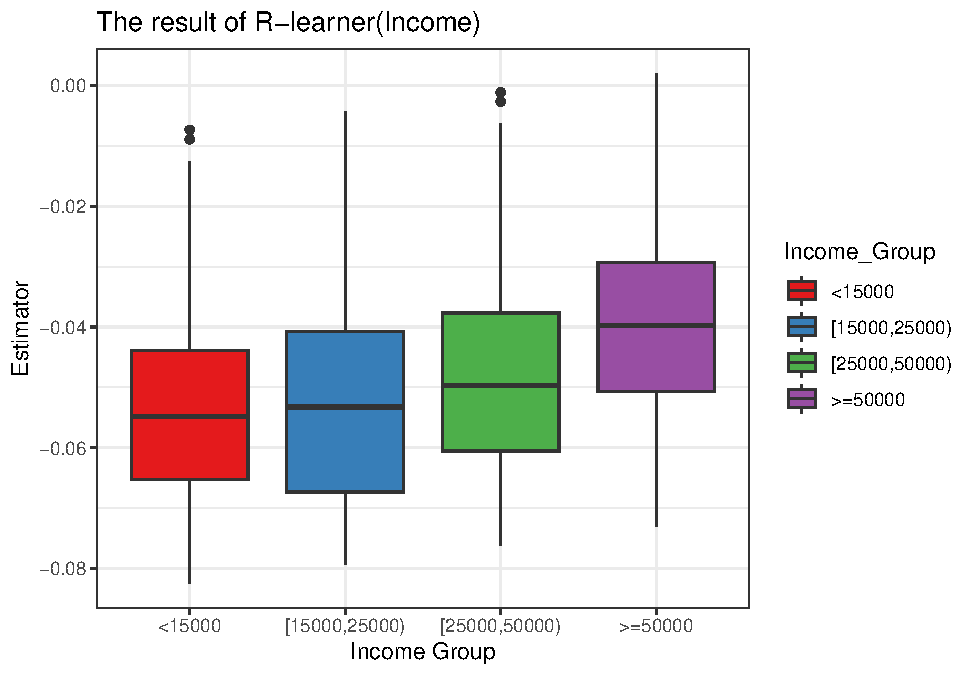
\includegraphics{template_files/figure-latex/unnamed-chunk-7-1.pdf}
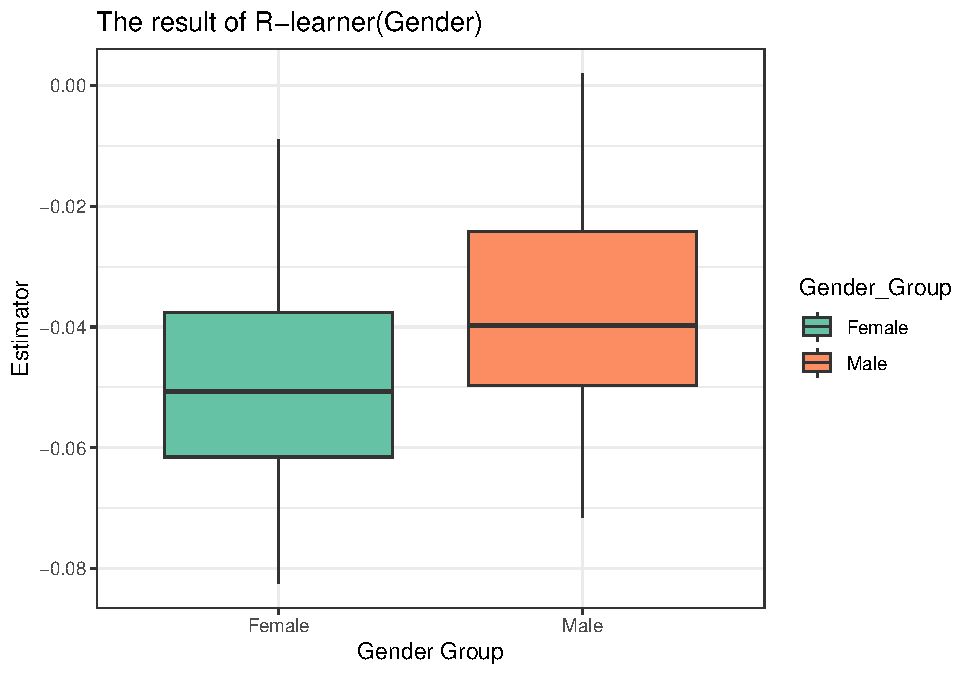
\includegraphics{template_files/figure-latex/unnamed-chunk-7-2.pdf}
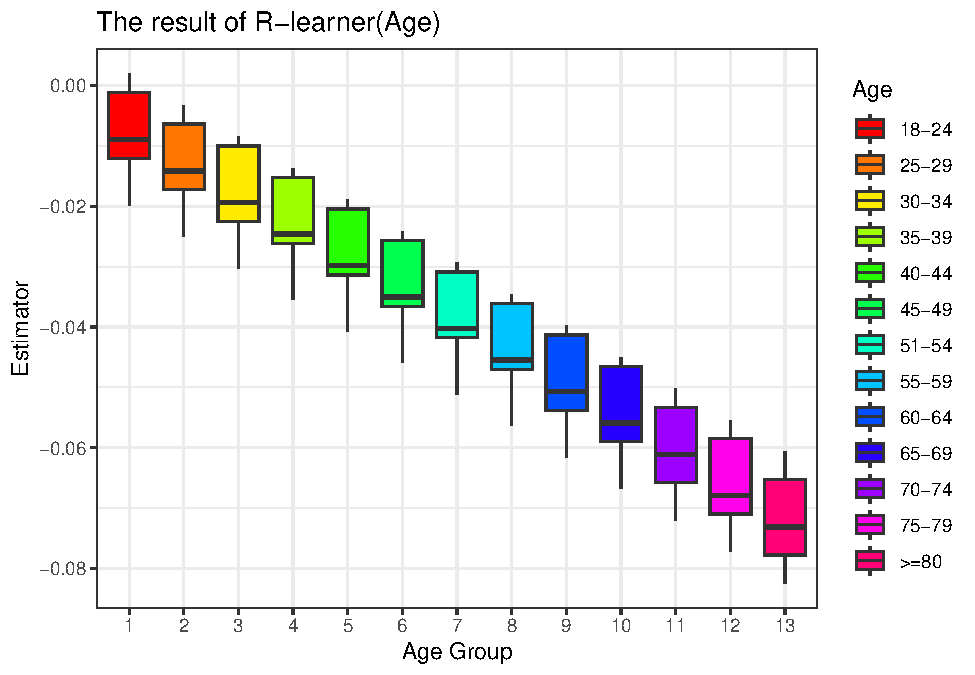
\includegraphics{template_files/figure-latex/unnamed-chunk-7-3.pdf}

\hypertarget{results}{%
\subsection{Results}\label{results}}

From the R-learner plots, we discern that higher income individuals are
less likely to develop diabetes, even have poor lifestyle choices. This
pattern is particularly noticeable for those earning over \$50,000
annually. Regarding gender, the difference in diabetes risk between good
and poor lifestyle habits is more pronounced in females than males,
underscoring the importance of healthy habits for women. In terms of
age, the substantial variation in CATE across different age groups
suggests that maintaining a healthy lifestyle becomes increasingly vital
as one ages. This is because poor lifestyle choices are more likely to
induce diabetes as age increases.

\hypertarget{discussion}{%
\subsection{Discussion}\label{discussion}}

{[}Discuss the implications and significance of the findings, relate
them to the research questions/hypotheses, and address any limitations
or potential sources of bias.{]}

\hypertarget{conclusion}{%
\subsection{Conclusion}\label{conclusion}}

{[}Summarize the key takeaways from the study and suggest possible
avenues for future research.{]}

\hypertarget{references}{%
\subsection{References}\label{references}}

{[}Include a list of cited references using a suitable citation style
(e.g., APA, MLA, IEEE).{]}

\newpage

\hypertarget{appendix}{%
\subsection{Appendix}\label{appendix}}

\end{document}
